\documentclass[aps,prb,10pt,endfloats]{revtex4-1}
\usepackage{amsmath}
\usepackage{framed}
\usepackage{color}
\usepackage{graphicx}
\usepackage[caption=false]{subfig}
\usepackage[backref,colorlinks,linkcolor=blue,citecolor=blue,urlcolor=blue]{hyperref}
% \usepackage{fullpage}
\usepackage{parskip}

\definecolor{shadecolor}{rgb}{0.757, 0.882, 0.925}

\begin{document}

\noindent Dr. Jason T. Haraldsen\hfill{\today}\\
Assistant Editor\\
Physical Review B\\

\noindent Dear Dr. Haraldsen,\\

Attached is the revised version of our paper entitled \emph{Plasmon dispersion
in graphite: A comparison of current ab initio methods}, manuscript
BZ13264/Anderson. We thank the referees for their useful comments and
suggestions, as they have helped us to significantly improve the quality of our
work.\\

In the following, we answer all the points raised by the referees and list all
the changes made to the paper. We have marked changes in red for easy reference
in the revised PDF version of the manuscript. Our responses to the reviewer
comments are enclosed in blue boxes below.\\

We are confident that all suggestions have been met and hope that our manuscript
is now acceptable for publication in Physical Review B.\\

\noindent Best regards,\\

\noindent Dr. Sean M. Anderson\\
\href{mailto:sma@cio.mx}{sma@cio.mx}

%%%%%%%%%%%%%%%%%%%%%%%%%%%%%%%%%%%%%%%%%%%%%%%%%%%%%%%%%%%%%%%%%%%%%%%%%%%%%%%%
%%%%%%%%%%%%%%%%%%%%%%%%%%%%%%%%%%%%%%%%%%%%%%%%%%%%%%%%%%%%%%%%%%%%%%%%%%%%%%%%

\section{Report of the First Referee -- BZ13264/Anderson}

Anderson and colleagues present a theoretical study of the momentum dependent
EELS on graphite, comparing their results with published experimental data. The
work compares three methods, BSE, ALDA, and RPA, assuming the same starting band
structure, and investigates also the effect of the neglect of coupling between
positive and negative energy e-h pairs (Tamm-Dancoff approximation). The main
conclusions are that in graphite BSE gives the best results and the coupling
term is important. The paper is clearly written, although somewhat repetitive in
parts and somewhat long considering many of the points mentioned have been
discussed in previous works and several similar calculations have been reported
elsewhere (the references given appear adequate).
\begin{shaded*}
Thank you for your assessment.\\

In order to minimize some of the repetitive discussion, we have shortened the
length of the manuscript by 3 pages by moving Section IV B (regarding the $\pi +
\sigma$ plasmon) and Appendix A (computational benchmarks) to the new
Supplemental Material, and by removing Fig. 8 which added very little to the
overall message of the article.
\end{shaded*}

As the authors note, the work is a ``systematic study'' on a ``benchmark
material''. However, the conclusions drawn about coupling may be relevant only
for a semi-metal like graphite, a material which is of limited interest nowadays
in comparison to its 2D counterpart (the TDA appears to work well in other
materials like BN, for instance). It is also disappointing that the authors do
not discuss the different plasmon dispersions, in particular, their BSE-CP data
appears linear (Fig. 4) instead of the measured parabolic behavior in $q$, while
other approximations appear to yield the correct dispersion.
\begin{shaded*}
Graphite was selected as our material of study due to the relatively large
quantity of available experimental data that is quite consistent (almost 5
decades worth). It also happens to be a plasmonic material where the TDA does
not yield spectra that closely match experimental measurements. Graphene is also
a semi-metal, so even if these results are indeed limited to only semi-metals,
they would still be applicable.\\

However, 2D systems (such as graphene) often pose significant computational
challenges, such as the application of the Coulomb cutoff to the electronic
screening, and the large supercell volumes required to eliminate the spurious
interlayer interactions. We have experience with GW calculations for a variety
of bulk and 2D materials, such as graphane/graphone, $\textrm{MoS}_{2}$ and
$\textrm{In}_{2}\textrm{Se}_{3}$; these calculations are often very difficult
(or impossible) to converge. Again, we consider bulk graphite to be a good
platform with which to consistently test these theoretical methods.

The apparent linear behavior of the $q$ dispersion was caused by an error on our
part, which is explained in detail in point 2 below. Now that we have corrected
that error, we obtain the correct quadratic dispersion relation. We have added a
curve to Fig. 5 in the main manuscript to demonstrate this behavior.\\

We have also toned down the language in the article in order to more accurately
convey the results of the work.
\end{shaded*}

Other specific points:

\begin{enumerate}

\item
Both Ref 65 [Marinopoulos 2004, Fig 10] and Ref 51 [Liou, Fig 5c,d] report EELS
calculations on graphite within RPA and ALDA. The agreement with experiment in
those works is quite perfect. Instead, the present work, with the same
approximations, yields worse agreement.
\begin{shaded*}
In our opinion, there are two potential explanations for this disagreement:
convergence and eigen-energies.

\emph{Concerning convergence}: attached to this document, we supply a
convergence report for the TDDFT RPA calculation, for three distinct values of
transferred momentum $q$. We find that our results are well converged for almost
all parameters, with the exception of \textbf{k}-points for $q$ values that are
far beyond the first Brillouin zone. However, these large values of $q$ do not
even factor into our plasmon dispersion analysis of Figs. 4, 5, and 7, so the
lack of convergence in such cases does not change our final results.
Additionally, the \textbf{k}-point grids have a serious impact on every result
presented, as they not only determine convergence but also the available values
of $q$ that can be probed; the selected 12$\times$12$\times$02 and
14$\times$14$\times$02 grids offer a good compromise between convergence and
available $q$ values. Liou et al., for instance, use a very fine
\textbf{k}-point grid of 40$\times$40$\times$14, but with a cutoff energy of
less than 8\,Ha, as opposed to the 20\,Ha we use here.

\emph{Concerning eigen-energies}: Fig. 3 of our manuscript clearly demonstrates
that the application of a correction to the DFT eigen-energies can have a
significant impact on the peak position and intensity. Liou et al. make no
specific mention of any type of correction being applied to their calculated
eigen-energies; thus, we cannot readily assume that they have carried out some
type of quasiparticle correction to their base eigen-energies. On the other
hand, Marinopoulos et al. mention that the valence bandwidth from photoemission
data is stretch by 11\,\% with respect to the DFT results, and that GW
calculations bring the DFT band structure into much better alignment with the
experimental results. As these corrections are indeed necessary to accurately
describe the observed spectra, we have applied stretching values obtained from
GW calculations to our eigen-energies. It is also worth noting that our
stretching values were calculated by one of the authors of that article.

Therefore, we are confident that the results presented in this work are
thoroughly converged, and that the stretched eigen-energies do play a
significant role in providing accurate peak positions across all methods.
\end{shaded*}

\item
The author's data at $q\rightarrow0$ seems out of step with the $q>0$ data,
clearly shown in Fig. 6, and in Fig. 4. This makes it harder to judge the
dispersion. Is there a problem of convergence, or of methodology? Are the EELS
peak positions determined from the eigenvalues or from the broadened curves?
\begin{shaded*}
This discrepancy is due to an error on our part, and we thank the reviewer for 
pointing this out (we should have not made this mistake): we selected the 
wrong column when extracting the peak positions for the spectra at $q=0.00$ 
for all methods.

In all $\mathbf{q}\ne 0$, our files contain two columns: the energy loss and the
EELS signal $\epsilon_{M}^{-1}(\omega)$. Only the $\mathbf{q}=0$ case contains
nine columns: the energy loss and the value of
$\epsilon_M^{-1}(\mathbf{q},\omega)$ for different directions of $\mathbf{q}\to
0$: along the $x, y, z$ Cartesian coordinates, along
$\mathbf{b}_{1},\mathbf{b}_{2},\mathbf{b}_{3}$ reciprocal lattice primitive
vectors, and the averages.

Fig. \ref{fig:columns} depicts the results for the different available columns;
$r$ and $c$ are reciprocal and Cartesian averages. The out-of-plane response
corresponds to the $b_{3} = z$ direction, and does not play any part in this
study, where we are probing along in-plane paths. The previous wrong result,
taking the default second column corresponding to the average along the
reciprocal directions, was strongly biased in both intensity and peak position
by the influence of the out-of-plane component (in a cubic material this would
have not biased the result at all). By selecting the spectra for the
$\mathbf{b}_{1}$ direction (correspondent to the $\Gamma\to\mathrm{M}$
direction), we restore the correct result for the $\mathbf{q} = 0$ case.

In Fig. \ref{fig:disp}, we present the EEL spectra for values of $q$ along the
$\Gamma\rightarrow\mathrm{M}$ path. We have selected small values of $q$,
calculated with a fine 40$\times$40$\times$02 \textbf{k}-point grid. Comparing
the $q=0.00$ curve plotted from column 2 (averaged) and column 4 (along the
$\mathbf{b}_{1}$ direction, which corresponds to the $\Gamma\to\mathrm{M}$
direction), we see that the latter is much more representative of the $q$
dispersion behavior. As mentioned above, this does not affect any of the
calculations for $q > 0$.

After choosing the appropriate column for the spectra at $q=0.00$, we see that
the plasmon dispersion does indeed have quadratic behavior. We have corrected
every figure in the main manuscript involving these results.
\end{shaded*}

\begin{figure}[t]
\centering
\subfloat[The different directions, both in the reciprocal lattice and Cartesian
spaces.\label{fig:columns}]
{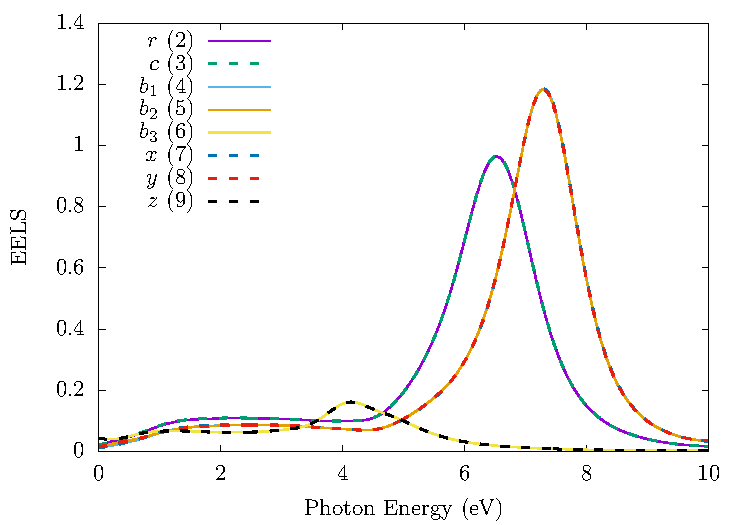
\includegraphics[width=0.4\linewidth]{figures/smallq-eels.pdf}}
~
\subfloat[EEL spectra for small values of $q$; $q=0.00$ is plotted from an
average across all directions (column 2) and along the $\mathbf{b}_1$ in-plane
direction (column 4).\label{fig:disp}]
{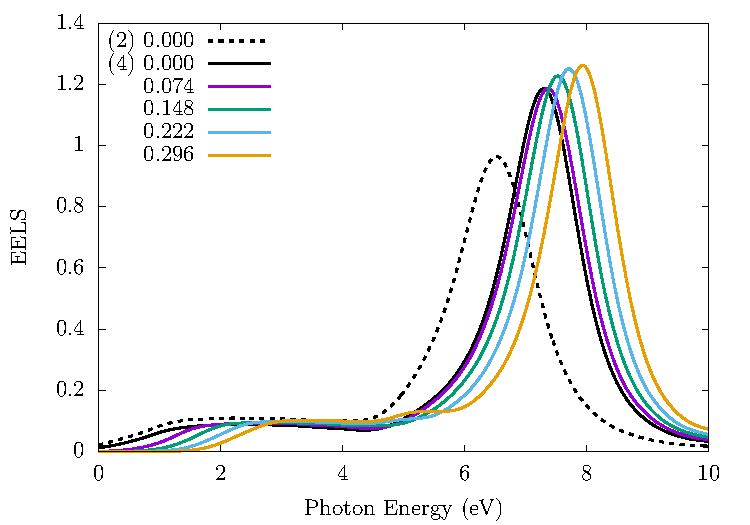
\includegraphics[width=0.4\linewidth]{figures/smallq-disp.pdf}}
\caption{}
\label{fig:eels}
\end{figure}


\item
I am skeptical about the authors claims regarding the peak intensity (IV A)
comparison with experiment since their broadening is very large (0.6eV); again,
previous works found more reasonable intensities within RPA and ALDA. These
three points in fact suggest a lack of convergence in the authors' calculations.
While I appreciate that BSE-CP is a very tough calculation, it is unfortunately
a serious point in a work whose main message requires a careful comparison of
different approaches.
\begin{shaded*}
Concerning broadening and previous works,
\begin{itemize}
\item Marinopoulos et al. uses a broadening of 0.5\,eV (see caption of Fig. 6).
\item Liou et al. does not explicitly mention any particular broadening value
but the curves look just as broadened as, or even more than, Marinopoulos et al.
\item Trevisanutto et al. (Ref. 49) present several results for Im
$\epsilon(\omega)$ for graphite; the in plane absorption spectra featured in
Fig. 1 use a relative Gaussian broadening of $\sigma = 0.075\omega$, which puts
the broadening at very comparable values in the $\pi$ plasmon energy range of
$\sim$6--10\,eV.
\end{itemize}

We do not think that our value of 0.6\,eV is particularly large in light of
these previous works. In the attached convergence report, we have used a smaller
broadening of 0.25\,eV. Comparing the spectra intensity between the two
broadenings, we obtain average percent differences below 20\,\% for every
point.

Therefore, any differences between the results presented in this work, and those
previously reported in the literature are more likely due to convergence
discrepancies or from the eigen-values used, as mentioned in the points above.
We agree with the reviewer when saying that the intensity clearly depends on
the broadening, but our claim about the importance of including coupling effects 
for a better description of the intensity of the peaks still holds; it is valid
not only for the BSE, but also for RPA or ALDA.
\end{shaded*}

\end{enumerate}

In summary, although the paper has appeal as a reference work, I have some
doubts about the numerical convergence of some of the data, much of the physics
``message'' has been published elsewhere, the novel features are quite limited
in scope being related mostly to methodology.
\begin{shaded*}
Thank you for your shrewd observations and very useful comments. We strove for
this work to be a relatively complete, self-contained reference on the
application of these theoretical frameworks on a well-characterized material.
Specifically, we have
\begin{itemize}
\item Shortened the length of the main manuscript by 3 pages,
\item Demonstrated that our calculations are adequately converged (see attached
convergence report),
\item Cited most of the relevant literature, both for theoretical developments
and experimental measurements,
\item Toned down the language to better convey the results and conclusions, and
finally
\item Expanded our Theory section in order to present a more complete reference
for the reader.
\end{itemize}

With these changes, we hope that this paper can serve as an important reference
material for researchers working in related fields.
\end{shaded*}


%%%%%%%%%%%%%%%%%%%%%%%%%%%%%%%%%%%%%%%%%%%%%%%%%%%%%%%%%%%%%%%%%%%%%%%%%%%%%%%%
%%%%%%%%%%%%%%%%%%%%%%%%%%%%%%%%%%%%%%%%%%%%%%%%%%%%%%%%%%%%%%%%%%%%%%%%%%%%%%%%

\section{Report of the Second Referee -- BZ13264/Anderson}

The paper ``Plasmon dispersion in graphite: A comparison of current ab initio
methods'' by Sean M. Anderson, Bernardo S. Mendoza, Giorgia Fugallo, and
Francesco Sottile presents a comparison of different numerical methods to
determine the dielectric function and EELS spectrum of a solid. The techniques
are applied to the calculation of the plasmon spectrum of graphite and compared
to experimental results obtained over the past several decades to serve as a
benchmark for the use of these methods for future systems. The methods include
TDDFT, adiabatic LDA (ALDA), RPA and the solution of the Bethe-Salpeter equation
(BSE). They also compare the full method including interactions between excitons
with the Tamm-Dancoff approximation.

The article is a careful study of involved methods applied to a well-known
system. As such, it is worth publishing as it may serve as a reference for
calculations made on new materials. Overall the article is well written, but a
few revisions are needed before the article can be accepted for publication in
Physical Review B.
\begin{shaded*}
Thank you for your assessment and helpful suggestions. We have integrated these
suggestions into the manuscript as follows below.
\end{shaded*}

\begin{enumerate}

\item
The second half of the abstract should be more explicit about the results of the
article (TD is not good, BSE good but time-consuming, etc.) Also, the abstract
has the statements ``We accurately discern'' and ``We accurately compare''. What
does ``accurately'' mean in this context? What does ``discern'' mean in this
context?
\begin{shaded*}
We have expanded on the abstract to include a more explicit description of the
results and improved some of the phrasing therein.
\end{shaded*}

\item
The introduction describes the methods and difficulties related to the
calculation of optical spectra in solids. The paper then states that it compares
these methods as they apply to graphite. There is not much new physics but the
paper focuses on a comparison of methods. What is unclear in the introduction is
if the authors were motivated to do their study by a present-day physical
problem or system. Was the main interest only to compare different numerical
methods? Or was it to study the plasmon spectrum of graphite? In short, the
introduction should be more explicit about the underlying motivation. It would
also have been desirable to apply the methods to a novel material that is
presently under investigation.
\begin{shaded*}
We have added a sentence to the second-to-last paragraph of the Introduction
(page 2) with a clear statement of our motivation.
\end{shaded*}

\item
There is a typo on the left hand side of Eq. (8).
\begin{shaded*}
In the new revision of the manuscript, Eq. (8) is now Eq. (3); we have corrected
the left hand side, changing $\epsilon_{\mathrm{M}}(\mathbf{q},
\omega)$ to $\epsilon^{-1}_{\mathrm{M}}(\mathbf{q}, \omega)$.
\end{shaded*}

\item
When describing the results of Fig. 3, the authors state ``however, the nature
of the stretching causes a redistribution of the band energies, which causes
changes in both the peak position and intensities.'' The statement should be
qualified: is the redistribution improving or worsening the description of the
EEL spectrum?
\begin{shaded*}
The stretched band energies definitely improve the agreement between the
theoretical and experimental peak positions. The reason is that the stretching simulates 
the correct band structure, as it would be experimentally given by photo-emission 
spectroscopy. We have added a sentence at the end
of the paragraph (second-to-last paragraph of page 6) that clarifies this.
\end{shaded*}

\item
In the description of Fig. 5 the authors compare their results with the
``Zeppendfeld'' and ``Liou'' data and state that they are closer to the former.
What conclusion can be drawn from that observation?
\begin{shaded*}
After reviewing both references, we were not able to find any relation between
the two experiments and this observation. As it does not contribute anything to
the discussion, we have removed the phrase entirely.
\end{shaded*}

\item
The figure captions should be more elaborate and self-explanatory. When reading
them, one should be guided to the important features of the figure. For Figs. 6,
8, 9, 10 it would be useful to have a column label (either above or below the
column) that specifies ``with coupling'' and ``without coupling'' (the authors
will likely have a better keyword).
\begin{shaded*}
We have revised and expanded the captions of 9 figures to improve their
comprehension.
\end{shaded*}

Once the above points have been addressed, the paper can be recommended for
publication.
\begin{shaded*}
Again, thank you for the very useful feedback. Besides the corrections and
additions made above, we have also included a slightly expanded Theory section
to make the entire work more self-enclosed. We also reduced the length of the
paper by moving some content to a new Supplemental Material.

With these changes, we hope that this paper can serve as an important reference
material for researchers working in related fields.
\end{shaded*}

\end{enumerate}

\end{document}
